Микроконтроллер (англ. \textit{Micro Controller Unit, MCU}) --- микросхема, предназначенная для управления электронными устройствами \cite{wiki:microcontroller}. Типичный микроконтроллер сочетает на одном кристалле функции процессора и периферийных устройств, содержит ОЗУ и (или) ПЗУ. По сути, это однокристальный компьютер, способный выполнять относительно простые задачи. Микроконтроллер общается с внешним миром считывая значения на своих <<входах>> и выдавая соответствующие значения на своих <<выходах>>.

Общая структурная схема микроконтроллера представлена на рисунке~\ref{fig:microstruct}.

\begin{figure}[ht]
    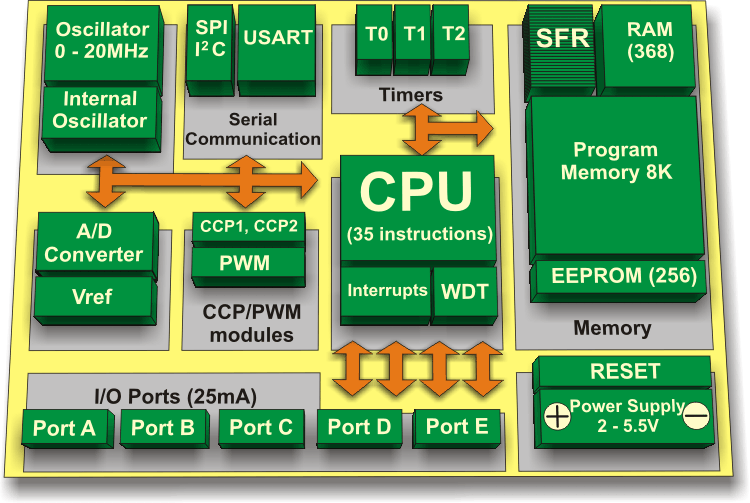
\includegraphics[width=.7\linewidth]{Figures/microstruct.png}
    \caption{Обобщённая структурная схема микроконтроллера}
    \label{fig:microstruct}
\end{figure}

Здесь можно наблюдать:

\begin{itemize}
    \item генератор задающей частоты (clock);
    \item последовательный UART-порт коммуникации с другими устройствами (например, по протоколу modbus);
    \item низкоуровневые таймеры (работающие на частотах начиная от задающей частоты и ниже);
    \item процессор с поддержкой прерываний;
    \item модуль широтно-импульсной модуляции;
    \item ЦАП/АЦП;
    \item порты ввода-вывода (аналоговые и цифровые);
    \item блок оперативной (RAM) и постоянной (EEPROM) запоминающей памяти.
\end{itemize}

Зачастую, частота работы микроконтроллеров недостаточна для обеспечения необходимой разрешающей способности Time of Flight устройства, и прибегают к \textbf{микропроцессорным} средствам, например платам на ARM-процессорах. Однако для целей моделирования был взят микроконтроллер ATMega, а точнее --- плата разработки Arduino, использующая в своём ядре микроконтроллер ATMega.
